% \iffalse meta-comment
%
% Copyright (C) 2015 by Tibor Tomacs
%
% This file may be distributed and/or modified under the
% conditions of the LaTeX Project Public License, either version 1.2
% of this license or (at your option) any later version.
% The latest version of this license is in:
%
% http://www.latex-project.org/lppl.txt
%
% and version 1.2 or later is part of all distributions of LaTeX
% version 1999/12/01 or later.
%
% \fi
%
% \iffalse
%<*driver>
\ProvidesFile{bookcover.dtx}
\newcommand{\eifiledate}{2015/03/04}
\newcommand{\eifilever}{v1.0}
%</driver>
%<class>\NeedsTeXFormat{LaTeX2e}[1999/12/01]
%<class>\ProvidesClass{bookcover}[2015/03/04 v1.0 class for book covers and dust jackets]
%
%<*driver>
\documentclass[a4paper]{ltxdoc}
\usepackage[utf8]{inputenc}
\usepackage[T1]{fontenc}
\usepackage[paperwidth=210mm,paperheight=295mm,width=160mm,top=25mm,bottom=25mm,outer=25mm]{geometry}
\usepackage[unicode,pdfstartview=FitH,bookmarksnumbered,pdfborder={0 0 0},colorlinks,linktocpage,pagecolor=blue,linkcolor=blue,urlcolor=blue,]{hyperref}
\usepackage[english]{babel}
\usepackage{xcolor,graphicx,listings}
\lstset{
literate={ü}{{\"u}}1{ó}{{\'o}}1{é}{{\'e}}1{á}{{\'a}}1{Á}{{\'A}}1,
basicstyle=\color{example}\small\ttfamily,
columns=fullflexible,
comment=[l][\ttfamily\color{black}]{\%}}
\colorlet{newcommand}{red!50!black}
\colorlet{example}{blue!50!black}
\colorlet{layer}{green!50!black}

\begin{document}
    \DocInput{./bookcover.dtx}
\end{document}
%</driver>
% \fi
%
% \CheckSum{1182}
%
% \CharacterTable
% {Upper-case \A\B\C\D\E\F\G\H\I\J\K\L\M\N\O\P\Q\R\S\T\U\V\W\X\Y\Z
%     Lower-case \a\b\c\d\e\f\g\h\i\j\k\l\m\n\o\p\q\r\s\t\u\v\w\x\y\z
%     Digits \0\1\2\3\4\5\6\7\8\9
%     Exclamation         \!     Double quote    \"     Hash (number)   \#
%     Dollar              \$     Percent         \%     Ampersand       \&
%     Acute accent        \'     Left paren      \(     Right paren     \)
%     Asterisk            \*     Plus            \+     Comma           \,
%     Minus               \-     Point           \.     Solidus         \/
%     Colon               \:     Semicolon       \;     Less than       \<
%     Equals              \=     Greater than    \>     Question mark   \?
%     Commercial at       \@     Left bracket    \[     Backslash       \\
%     Right bracket       \]     Circumflex      \^     Underscore      \_
%     Grave accent        \`     Left brace      \{     Vertical bar    \|
%     Right brace         \}     Tilde           \~}
%
% \GetFileInfo{bookcover.cls}
%
% \title{Class for book covers and dust jackets\\
%        \textsf{bookcover.cls}\\
%        {\large\eifilever}}
% \author{Tibor Tómács\\
%         {\color{blue}\normalsize\href{mailto:tomacs@ektf.hu}{\nolinkurl{tomacs@ektf.hu}}}}
% \date{March 4, 2015}
% \maketitle
%
% \tableofcontents
%
% \section{Book cover parts and sizes}
% In the following picture we can see a tipical dust jacket. Its main parts are back flap, back, spine, front and front flap. 
% Typographically, a book cover is a dust jacket without flaps, the only difference is that the book cover is a fixed part of the book, whereas the dust jacket is removable.
% \begin{center}
% 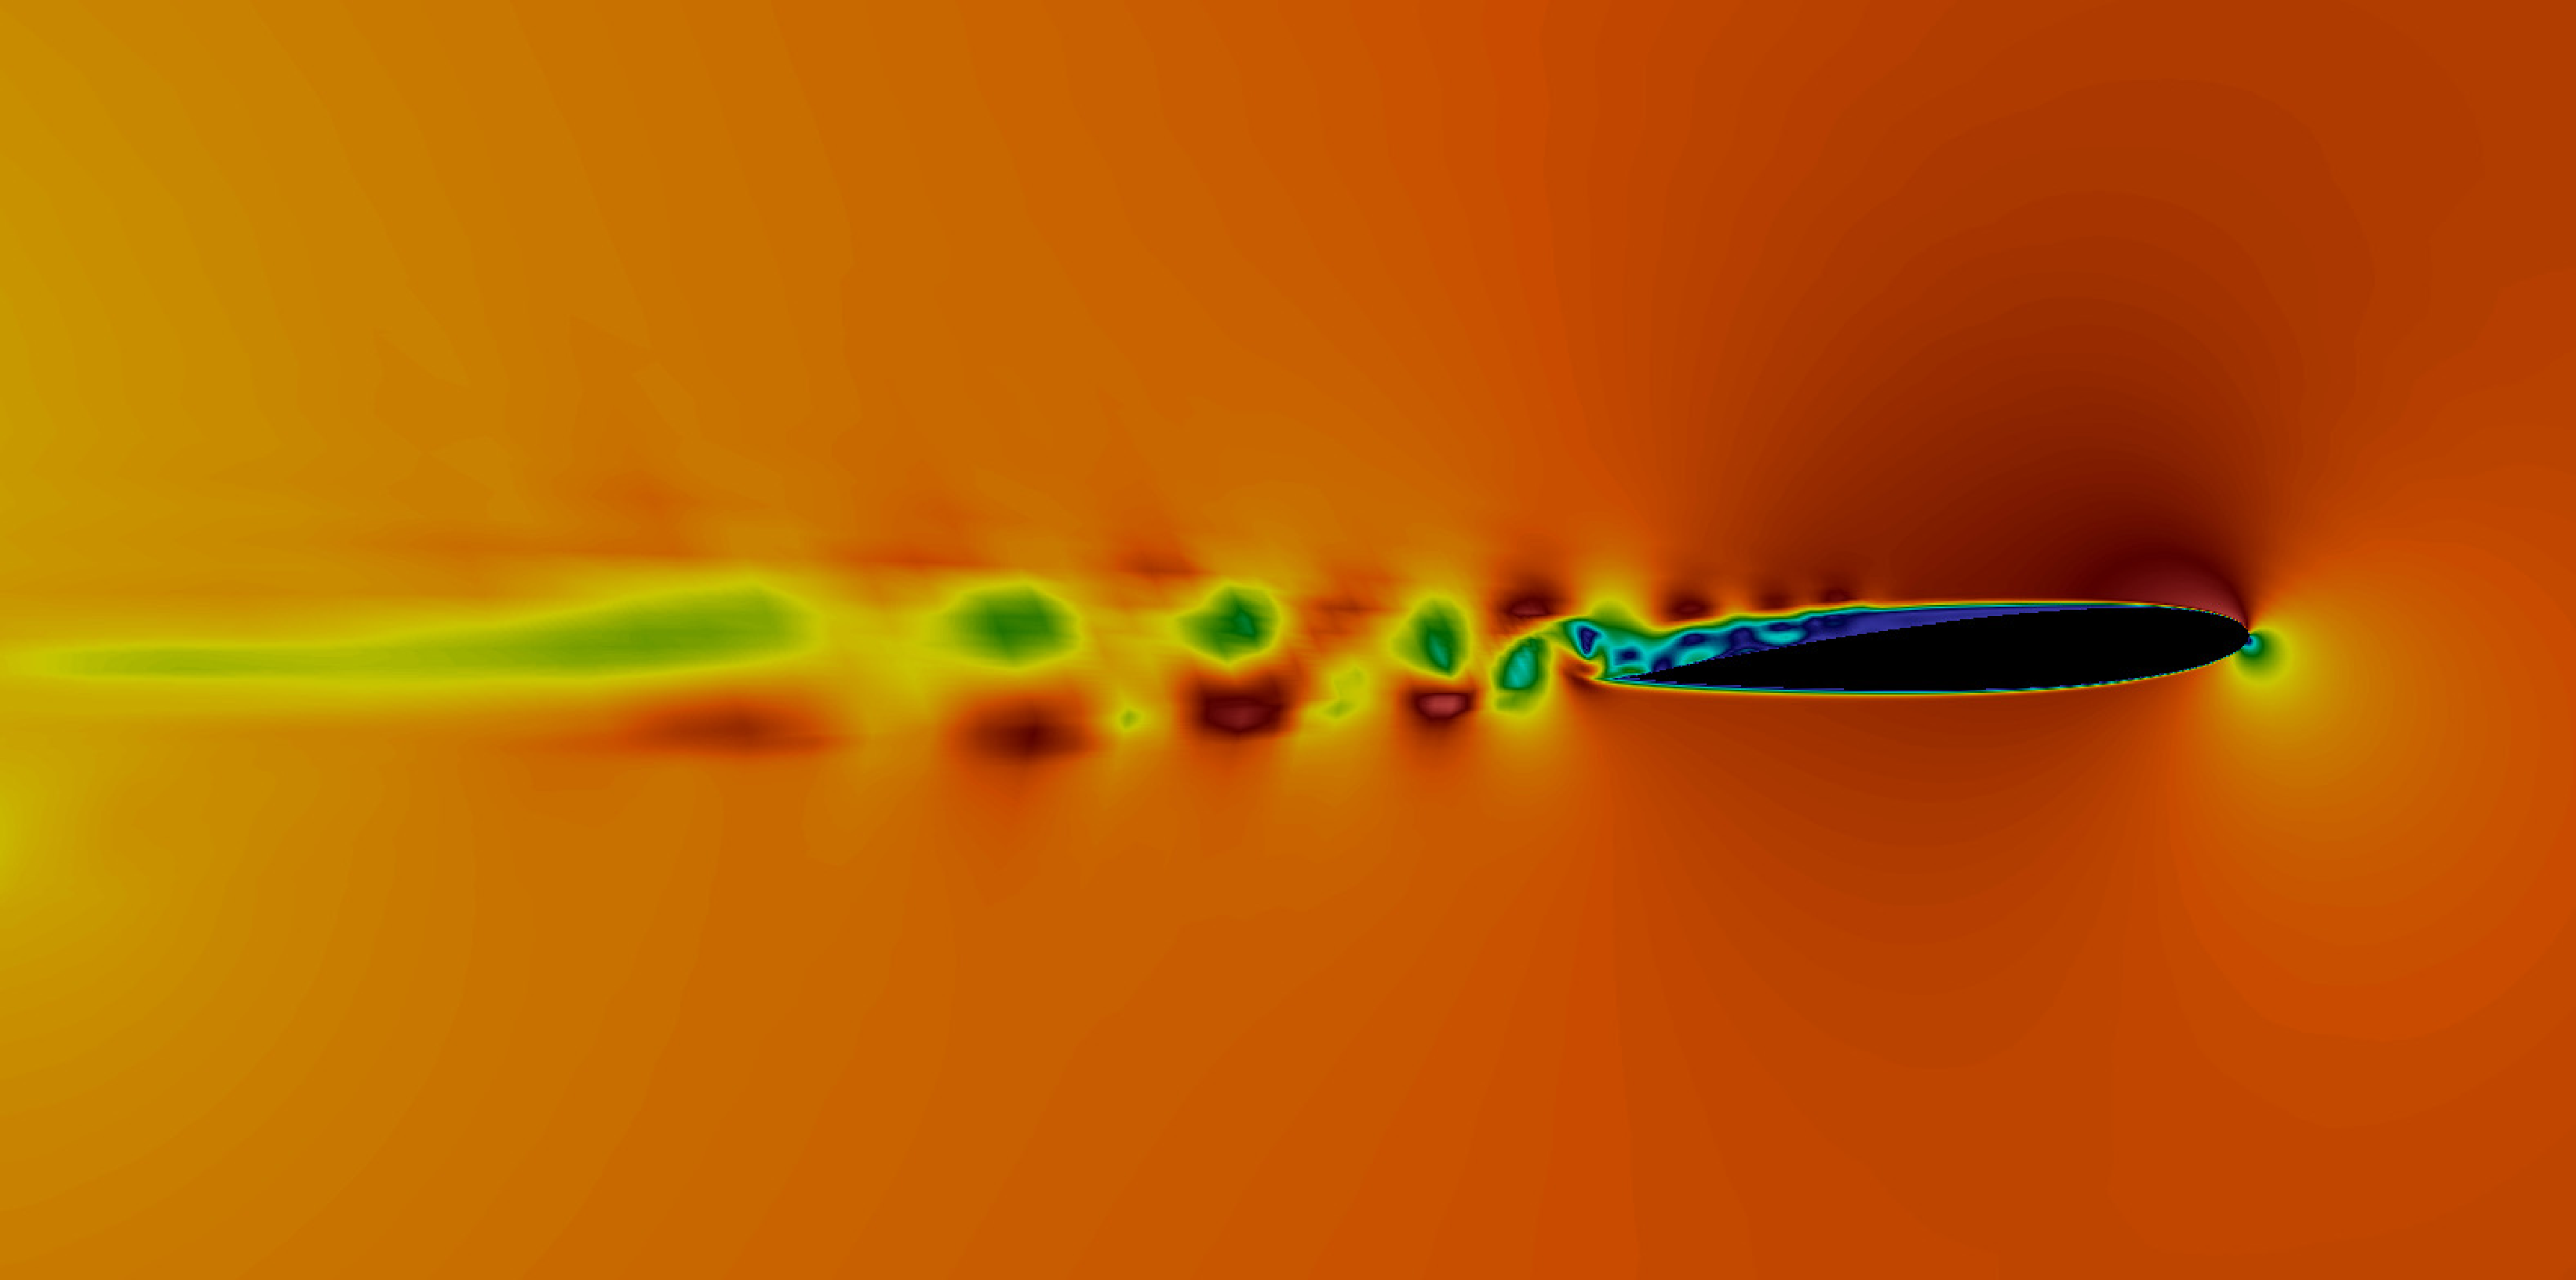
\includegraphics{figures/cover}
% \end{center}
% When we prepare a cover for printing, some marks are needed to know where to trim or fold the paper. These marks determine a special area of the sheet, which is called ``bleed'' (see the next figure). The background will be expanded onto the bleed, taking account of slight inaccuracy when trimming.
% \begin{center}
% \includegraphics{figures/coverscheme}
% \end{center}
%
% \subsection{Sizes}\label{subsec:sizes}
% We have to give the following sizes to prepare a cover: \texttt{coverwidth}, \texttt{coverheight}, \texttt{spinewidth}, \texttt{flapwidth}, \texttt{marklength}, \texttt{bleedwidth}.
% \begin{center}
% \includegraphics{figures/sizes}
% \end{center}
%
% \subsection{Trimmed version}\label{subsec:trimmed}
% After trimming we get the following result:
% \begin{center}
% \includegraphics{figures/result}
% \end{center}
%
% \subsection{Background parts}\label{subsec:background}
% Important: The bleed is a part of the background!
%
% \medskip\noindent
% In case |flapwidth>0mm| 
% \begin{center}
% \includegraphics{figures/background1}\\[4mm]
% \includegraphics{figures/background2}\\[4mm]
% \includegraphics{figures/background3}
% \end{center}
% In case |flapwidth=0mm| 
% \begin{center}
% \includegraphics{figures/background4}\\[4mm]
% \includegraphics{figures/background5}
% \end{center}
%
% \subsection{Foreground parts}\label{subsec:foreground}
% Important: The bleed is not part of the foreground!
%
% \medskip\noindent
% In case |flapwidth>0mm| 
% \begin{center}
% \includegraphics{figures/foreground1}
% \end{center}
% In case |flapwidth=0mm| 
% \begin{center}
% \includegraphics{figures/foreground2}
% \end{center}
%
% \section{Description}
%
% \subsection{Loading class}
% The class \texttt{bookcover} requires the services of the class \texttt{article} and the following packages:
% \texttt{kvoptions}, \texttt{geometry}, \texttt{graphicx}, \texttt{calc}, \texttt{xcolor}, \texttt{ifthen}, \texttt{tikz}, \texttt{eso-pic}, \texttt{textpos}.
%
% \bigskip\noindent
% Load the class as usual, with
%
% \medskip\noindent
% {\color{newcommand}|\documentclass|\oarg{options}|{bookcover}|}
%
% \begin{center}
% \begin{tabular}{@{}l@{\hspace*{-30mm}}r@{}} 
% \textbf{book cover size options} (see Subsection \ref{subsec:sizes}) & \textbf{default values}\\ 
% \hline  
% \texttt{coverwidth=}\meta{length}  & \texttt{170mm}\\ 
% \texttt{coverheight=}\meta{length} & \texttt{240mm}\\
% \texttt{spinewidth=}\meta{length}  &   \texttt{5mm}\\
% \texttt{flapwidth=}\meta{length}   &   \texttt{0mm}\\
% \texttt{marklength=}\meta{length}  &  \texttt{10mm}\\
% \texttt{bleedwidth=}\meta{length}  &   \texttt{5mm}\\
% &\\
% \textbf{other options}&\\ 
% \hline  
% \texttt{markthick=}\meta{length}   & thick of marks (default value: \texttt{0.4pt})\\
% \texttt{markcolor=}\meta{color}    & color of marks (default value: \texttt{red})\\
% \texttt{10pt}                      &   normal font size is 10\,pt (default)\\
% \texttt{11pt}                      &   normal font size is 11\,pt\\
% \texttt{12pt}                      &   normal font size is 12\,pt\\
% \texttt{grid}                      &   grid for checking sizes\\
% \texttt{trimmed}                   &   show trimmed version (see Subsection \ref{subsec:trimmed})
% \end{tabular} 
% \end{center}
% \bigskip\noindent\emph{Example:}
%\color{example}
%\begin{verbatim}
%\documentclass[flapwidth=50mm,spinewidth=15mm]{bookcover}
%\end{verbatim}
%\color{black}
%
% \subsection{Commands}
% This class defines two commands: 
%
% \medskip\noindent
% {\color{newcommand}|\setbookcover|\marg{main layer}\marg{part}\marg{content}}
%
% \medskip\noindent 
% \meta{main layer} (see the following subsubsections)\\ 
% \hspace*{10mm}\texttt{bgcolor}, \texttt{bgpic}, \texttt{bgtikz}, \texttt{fgfirst}, \texttt{fgsecond}
%
% \medskip\noindent The \meta{part} and the \meta{content} depend on the \meta{main layer} (see the following subsubsections).
%
% \medskip\noindent 
% {\color{newcommand}|\makebookcover|}
%
% \subsubsection{Background colors}
% {\color{newcommand}|\setbookcover{bgcolor}|\marg{background part}\marg{colors}}
%
% \medskip\noindent 
% \meta{background part} (see Subsection \ref{subsec:background})\\ 
% \hspace*{10mm}\texttt{back}, \texttt{front}, \texttt{spine}, \texttt{front flap}, \texttt{back flap}, \texttt{whole without flaps}, \texttt{whole}
%
% \medskip\noindent 
% \meta{colors} (options of command |\fill| of package \texttt{tikz})\\ 
% \hspace*{10mm}|color=|\meta{color name} (See \meta{color name} in the package \texttt{xcolor}.)\\ 
% \hspace*{10mm}|top color=|\meta{color name}\\ 
% \hspace*{10mm}|bottom color=|\meta{color name}\\ 
% \hspace*{10mm}|middle color=|\meta{color name}\\ 
% \hspace*{10mm}|inner color=|\meta{color name}\\ 
% \hspace*{10mm}|outer color=|\meta{color name}\\ 
% \hspace*{10mm}|ball color=|\meta{color name}\\ 
% \hspace*{10mm}|shading angle=|\meta{degrees} (This rotates the shading by the given angle.)
%
% \bigskip\noindent\emph{Example:}
%\color{example}
%\begin{verbatim}
%\setbookcover{bgcolor}{whole without flaps}{
%    top color=white, bottom color=blue!50!black, shading angle=60}
%\end{verbatim}
%\color{black}
%
% \subsubsection{Background pictures}
% {\color{newcommand}|\setbookcover{bgpic}|\marg{background part}\marg{picture file}}
%
% \medskip\noindent 
% \meta{background part} (see Subsection \ref{subsec:background})\\ 
% \hspace*{10mm}\texttt{back}, \texttt{front}, \texttt{spine}, \texttt{front flap}, \texttt{back flap}, \texttt{whole without flaps}, \texttt{whole}
%
% \medskip\noindent The picture will be rescaled according to the sizes of the current background part.
%
% \bigskip\noindent\emph{Example:}
%\color{example}
%\begin{verbatim}
%\setbookcover{bgpic}{front flap}{fig.png}
%\end{verbatim}
%\color{black}
%
% \subsubsection{Background Ti\emph{k}Z figures}
% {\color{newcommand}|\setbookcover{bgtikz}|\marg{background part}\marg{tikz code}}
%
% \medskip\noindent 
% \meta{background part} (see Subsection \ref{subsec:background})\\ 
% \hspace*{10mm}\texttt{back}, \texttt{front}, \texttt{spine}, \texttt{front flap}, \texttt{back flap}, \texttt{whole without flaps}, \texttt{whole}
%
% \medskip\noindent
% The Ti\emph{k}Z figure will be placed to the upper left corner of the current background part, without resizeing.
%
% \bigskip\noindent\emph{Example:}
%\color{example}
%\begin{verbatim}
%\setbookcover{bgtikz}{back}{
%    \fill[color=blue](0mm,250mm)--(100mm,250mm)--(100mm,245mm)--(0mm,110mm)--cycle;
%    \fill[color=yellow](5mm,5mm)--(175mm,245mm)--(175mm,0mm)--(5mm,0mm)--cycle;}
%\end{verbatim}
%\color{black}
%
% \subsubsection{First foreground}
% {\color{newcommand}|\setbookcover{fgfirst}|\marg{foreground part}\marg{content}}
%
% \medskip\noindent 
% \meta{foreground part} (see Subsection \ref{subsec:foreground})\\ 
% \hspace*{10mm}\texttt{back}, \texttt{front}, \texttt{spine}, \texttt{front flap}, \texttt{back flap}, \texttt{remark}
%
% \medskip\noindent The first foreground is the top layer of the book cover (see Subsection \ref{subsec:layers}).
%
% \bigskip\noindent\emph{Example:}
%\color{example}
%\begin{verbatim}
%\setbookcover{fgfirst}{spine}{
%    \vfill
%    \begin{center}
%        \rotatebox[origin=c]{90}{\bfseries Annales Mathematicae et Informaticae}
%    \end{center}
%    \vfill}
%\end{verbatim}
%\color{black}
%
% \subsubsection{Second foreground}
% {\color{newcommand}|\setbookcover{fgsecond}|\marg{foreground part}\marg{content}}
%
% \medskip\noindent 
% \meta{foreground part} (see Subsection \ref{subsec:foreground})\\ 
% \hspace*{10mm}\texttt{back}, \texttt{front}, \texttt{spine}, \texttt{front flap}, \texttt{back flap}
%
% \medskip\noindent The second foreground is under the first foreground (see Subsection \ref{subsec:layers}).
%
% \bigskip\noindent\emph{Example:} 
% The following code puts a picture behind the `TEXT' on the front cover:
%\color{example}
%\begin{verbatim}
%\setbookcover{fgsecond}{front}{
%    \vfill
%    \begin{center}
%        \includegraphics[width=80mm]{pic.png}
%    \end{center}
%    \vfill}
%\setbookcover{fgfirst}{front}{
%    \vfill
%    \begin{center}
%        TEXT
%    \end{center}
%    \vfill}
%\end{verbatim}
%\color{black}
%
% \subsubsection{Making book cover}
% {\color{newcommand}|\makebookcover|}
%
% \medskip\noindent 
% This command makes the book cover by using contents of background and foreground. 
%
% \subsection{Layers}\label{subsec:layers}
% In the following table we can see the hierarchy of the layers:
%
% \bigskip
% \begin{center}
% \begin{tabular}{@{}ll@{}c@{}}
% \cline{1-2} 
% |fgfirst|  & |back|, |front|, |spine|, |front flap|, |back flap|, |remark|& \color{layer}\emph{top layer}\\ 
% \cline{1-2}
% |fgsecond| & |back|, |front|, |spine|, |front flap|, |back flap|&\color{layer}$\uparrow$\\
% \cline{1-2}
% & |back|, |front|, |spine|, |front flap|, |back flap| &\color{layer}$\uparrow$\\
% |bgtikz| &  |whole without flaps| &\color{layer}$\uparrow$\\ 
% & |whole| &\color{layer}$\uparrow$\\
% \cline{1-2}
% & |back|, |front|, |spine|, |front flap|, |back flap| &\color{layer}$\uparrow$\\
% |bgpic| &  |whole without flaps| &\color{layer}$\uparrow$\\ 
% & |whole| &\color{layer}$\uparrow$\\
% \cline{1-2}
% & |back|, |front|, |spine|, |front flap|, |back flap| &\color{layer}$\uparrow$\\
% |bgcolor| &  |whole without flaps| &\color{layer}$\uparrow$\\ 
% & |whole| & \color{layer}\emph{bottom layer}\\
% \cline{1-2}
% \end{tabular} 
% \end{center}
% \bigskip\noindent For example, in case
%\color{example}
%\begin{verbatim}
%\setbookcover{bgpic}{whole}{fig1.jpg}
%\setbookcover{bgpic}{front}{fig2.jpg}
%\setbookcover{fgsecond}{front}{fig3.jpg}
%\setbookcover{fgfirst}{front}{TEXT}
%\end{verbatim}
%\color{black}
%the \texttt{TEXT} is above the \texttt{fig3.jpg}, the \texttt{fig3.jpg} is above the \texttt{fig2.jpg} and the \texttt{fig2.jpg} is above the \texttt{fig1.jpg}.
%
% \section{Examples}
% The first example is a dust jacket.
% \begin{center}
% \includegraphics[width=\textwidth]{example1}
% \end{center}
% \lstinputlisting{example1.tex}
%
% \noindent The second example is a two-sided book cover. The outside and the inside are edited in the same document.
% \begin{center}
% \includegraphics[page=1,width=\textwidth]{example2}\\[4mm]
% \includegraphics[page=2,width=\textwidth]{example2}
% \end{center}
% \lstinputlisting{example2.tex}
%
% \StopEventually{}
%
% \section{Implementation}
% 
%    \begin{macrocode}
%%
%% Options
\RequirePackage{kvoptions}
\SetupKeyvalOptions{family=bookcover,prefix=bookcover@}
\DeclareVoidOption{10pt}{\PassOptionsToClass{10pt}{article}}
\DeclareVoidOption{11pt}{\PassOptionsToClass{11pt}{article}}
\DeclareVoidOption{12pt}{\PassOptionsToClass{12pt}{article}}
\DeclareVoidOption{grid}{\PassOptionsToPackage{grid}{eso-pic}}
\DeclareStringOption[170mm]{coverwidth}
\DeclareStringOption[240mm]{coverheight}
\DeclareStringOption[5mm]{spinewidth}
\DeclareStringOption[0mm]{flapwidth}
\DeclareStringOption[10mm]{marklength}
\DeclareStringOption[.4pt]{markthick}
\DeclareStringOption[5mm]{bleedwidth}
\DeclareStringOption[red]{markcolor}
\DeclareBoolOption[false]{trimmed}
\ProcessKeyvalOptions{bookcover}

%% Loading class and packages
\LoadClass{article}
\RequirePackage{geometry,graphicx,calc,xcolor,ifthen,tikz,eso-pic}
\RequirePackage[absolute]{textpos}

%% Page style is empty
\pagestyle{empty}

%% New length commands
\newlength{\coverwidth}
\newlength{\coverheight}
\newlength{\spinewidth}
\newlength{\flapwidth}
\newlength{\marklength}
\newlength{\markthick}
\newlength{\bleedwidth}
\newlength{\bookcover@xpos@}
\newlength{\bookcover@ypos@}
\newlength{\bookcover@partwidth@}
\newlength{\bookcover@partheight@}

%% Set length commands
\setlength{\coverwidth}{\bookcover@coverwidth}
\setlength{\coverheight}{\bookcover@coverheight}
\setlength{\spinewidth}{\bookcover@spinewidth}
\setlength{\flapwidth}{\bookcover@flapwidth}
\setlength{\marklength}{\bookcover@marklength}
\setlength{\markthick}{\bookcover@markthick}
\setlength{\bleedwidth}{\bookcover@bleedwidth}
\setlength{\paperwidth}{2\marklength+2\bleedwidth+2\coverwidth+2\flapwidth+\spinewidth}
\setlength{\paperheight}{2\marklength+2\bleedwidth+\coverheight}
\setlength{\parindent}{0pt}

%% If grid is true, then mark thick is 2pt and mark color is red
\ifESO@grid\setlength{\markthick}{2pt}\def\bookcover@markcolor{red}\fi

%% Internal macros
\def\bookcover@xpos#1{\setlength{\bookcover@xpos@}{#1}}
\def\bookcover@ypos#1{\setlength{\bookcover@ypos@}{#1}}
\def\bookcover@partwidth#1{\setlength{\bookcover@partwidth@}{#1}}
\def\bookcover@partheight#1{\setlength{\bookcover@partheight@}{#1}}
\def\bookcover@bgcolor#1{
    \begin{textblock*}{\bookcover@partwidth@}(\bookcover@xpos@,\bookcover@ypos@)
        \tikz\expandafter\fill#1 (0mm,0mm) rectangle (\bookcover@partwidth@,\bookcover@partheight@);
    \end{textblock*}}
\def\bookcover@bgpic#1{
    \begin{textblock*}{\bookcover@partwidth@}(\bookcover@xpos@,\bookcover@ypos@)
        \includegraphics[width=\bookcover@partwidth@,height=\bookcover@partheight@]{#1}
    \end{textblock*}}
\def\bookcover@bgtikz#1{
    \begin{textblock*}{\bookcover@partwidth@}(\bookcover@xpos@,\bookcover@ypos@)
        \begin{tikzpicture}
            #1
        \end{tikzpicture}
    \end{textblock*}}
\def\bookcover@fg#1{
    \begin{textblock*}{\bookcover@partwidth@}(\bookcover@xpos@,\bookcover@ypos@)
        \parbox[t][\bookcover@partheight@][t]{\bookcover@partwidth@}{#1}
    \end{textblock*}}
\def\bookcover@vmark{
    \begin{textblock*}{\bookcover@partwidth@}(\bookcover@xpos@,\bookcover@ypos@)
        {\color{\bookcover@markcolor}\rule[0pt]{\markthick}{\marklength}}
    \end{textblock*}}
\def\bookcover@hmark{
    \begin{textblock*}{\bookcover@partwidth@}(\bookcover@xpos@,\bookcover@ypos@)
        {\color{\bookcover@markcolor}\rule[0pt]{\marklength}{\markthick}}
    \end{textblock*}}
\def\bookcover@reset{
    \def\bookcover@bgcolor@whole{}
    \def\bookcover@bgcolor@wholewf{}
    \def\bookcover@bgcolor@back{}
    \def\bookcover@bgcolor@front{}
    \def\bookcover@bgcolor@backflap{}
    \def\bookcover@bgcolor@frontflap{}
    \def\bookcover@bgcolor@spine{}
    \def\bookcover@bgpic@whole{}
    \def\bookcover@bgpic@wholewf{}
    \def\bookcover@bgpic@back{}
    \def\bookcover@bgpic@front{}
    \def\bookcover@bgpic@backflap{}
    \def\bookcover@bgpic@frontflap{}
    \def\bookcover@bgpic@spine{}
    \def\bookcover@bgtikz@whole{}
    \def\bookcover@bgtikz@wholewf{}
    \def\bookcover@bgtikz@back{}
    \def\bookcover@bgtikz@front{}
    \def\bookcover@bgtikz@backflap{}
    \def\bookcover@bgtikz@frontflap{}
    \def\bookcover@bgtikz@spine{}
    \def\bookcover@fgfirst@back{}
    \def\bookcover@fgfirst@front{}
    \def\bookcover@fgfirst@spine{}
    \def\bookcover@fgfirst@backflap{}
    \def\bookcover@fgfirst@frontflap{}
    \def\bookcover@fgfirst@remark{}
    \def\bookcover@fgsecond@back{}
    \def\bookcover@fgsecond@front{}
    \def\bookcover@fgsecond@spine{}
    \def\bookcover@fgsecond@backflap{}
    \def\bookcover@fgsecond@frontflap{}}
    
%% Reset datas
\bookcover@reset    
    
%% Definition of command \setbookcover    
\long\def\setbookcover#1#2#3{
    \ifthenelse{\equal{#1}{bgcolor}}{
        \ifthenelse{\equal{#2}{whole}}{\def\bookcover@bgcolor@whole{[#3]}}{}
        \ifthenelse{\equal{#2}{whole without flaps}}{\def\bookcover@bgcolor@wholewf{[#3]}}{}
        \ifthenelse{\equal{#2}{back}}{\def\bookcover@bgcolor@back{[#3]}}{}
        \ifthenelse{\equal{#2}{front}}{\def\bookcover@bgcolor@front{[#3]}}{}
        \ifthenelse{\equal{#2}{back flap}}{\def\bookcover@bgcolor@backflap{[#3]}}{}
        \ifthenelse{\equal{#2}{front flap}}{\def\bookcover@bgcolor@frontflap{[#3]}}{}
        \ifthenelse{\equal{#2}{spine}}{\def\bookcover@bgcolor@spine{[#3]}}{}}{}
    \ifthenelse{\equal{#1}{bgpic}}{    
        \ifthenelse{\equal{#2}{whole}}{\def\bookcover@bgpic@whole{#3}}{}
        \ifthenelse{\equal{#2}{whole without flaps}}{\def\bookcover@bgpic@wholewf{#3}}{}
        \ifthenelse{\equal{#2}{back}}{\def\bookcover@bgpic@back{#3}}{}
        \ifthenelse{\equal{#2}{front}}{\def\bookcover@bgpic@front{#3}}{}
        \ifthenelse{\equal{#2}{back flap}}{\def\bookcover@bgpic@backflap{#3}}{}
        \ifthenelse{\equal{#2}{front flap}}{\def\bookcover@bgpic@frontflap{#3}}{}
        \ifthenelse{\equal{#2}{spine}}{\def\bookcover@bgpic@spine{#3}}{}}{}    
    \ifthenelse{\equal{#1}{bgtikz}}{    
        \ifthenelse{\equal{#2}{whole}}{\def\bookcover@bgtikz@whole{#3}}{}
        \ifthenelse{\equal{#2}{whole without flaps}}{\def\bookcover@bgtikz@wholewf{#3}}{}
        \ifthenelse{\equal{#2}{back}}{\def\bookcover@bgtikz@back{#3}}{}
        \ifthenelse{\equal{#2}{front}}{\def\bookcover@bgtikz@front{#3}}{}
        \ifthenelse{\equal{#2}{back flap}}{\def\bookcover@bgtikz@backflap{#3}}{}
        \ifthenelse{\equal{#2}{front flap}}{\def\bookcover@bgtikz@frontflap{#3}}{}
        \ifthenelse{\equal{#2}{spine}}{\def\bookcover@bgtikz@spine{#3}}{}}{}     
    \ifthenelse{\equal{#1}{fgfirst}}{    
        \ifthenelse{\equal{#2}{back}}{\def\bookcover@fgfirst@back{#3}}{}
        \ifthenelse{\equal{#2}{front}}{\def\bookcover@fgfirst@front{#3}}{}
        \ifthenelse{\equal{#2}{spine}}{\def\bookcover@fgfirst@spine{#3}}{}
        \ifthenelse{\equal{#2}{back flap}}{\def\bookcover@fgfirst@backflap{#3}}{}
        \ifthenelse{\equal{#2}{front flap}}{\def\bookcover@fgfirst@frontflap{#3}}{}
        \ifthenelse{\equal{#2}{remark}}{\def\bookcover@fgfirst@remark{#3}}{}}{}    
    \ifthenelse{\equal{#1}{fgsecond}}{    
        \ifthenelse{\equal{#2}{back}}{\def\bookcover@fgsecond@back{#3}}{}
        \ifthenelse{\equal{#2}{front}}{\def\bookcover@fgsecond@front{#3}}{}
        \ifthenelse{\equal{#2}{spine}}{\def\bookcover@fgsecond@spine{#3}}{}
        \ifthenelse{\equal{#2}{back flap}}{\def\bookcover@fgsecond@backflap{#3}}{}
        \ifthenelse{\equal{#2}{front flap}}{\def\bookcover@fgsecond@frontflap{#3}}{}}{}}

%% Definition of command \makebookcover  
\def\makebookcover{
%% Background
\bookcover@ypos{\marklength}
\bookcover@partheight{\coverheight+2\bleedwidth}
%% {bgcolor}{whole}
\ifx\bookcover@bgcolor@whole\@empty\else
    \bookcover@xpos{\marklength}
    \bookcover@partwidth{2\coverwidth+2\bleedwidth+2\flapwidth+\spinewidth}
    \bookcover@bgcolor{\bookcover@bgcolor@whole}\fi
%% {bgcolor}{whole without flaps}
\ifx\bookcover@bgcolor@wholewf\@empty\else
    \ifdim\flapwidth>0mm
        \bookcover@xpos{\marklength+\bleedwidth+\flapwidth}
        \bookcover@partwidth{2\coverwidth+\spinewidth}
    \else
        \bookcover@xpos{\marklength}
        \bookcover@partwidth{2\coverwidth+2\bleedwidth+\spinewidth}\fi
    \bookcover@bgcolor{\bookcover@bgcolor@wholewf}\fi
%% {bgcolor}{back flap}
\ifx\bookcover@bgcolor@backflap\@empty\else\ifdim\flapwidth>0mm
    \bookcover@xpos{\marklength}
    \bookcover@partwidth{\flapwidth+\bleedwidth}
    \bookcover@bgcolor{\bookcover@bgcolor@backflap}\fi\fi
%% {bgcolor}{back}
\ifx\bookcover@bgcolor@back\@empty\else
    \ifdim\flapwidth>0mm
        \bookcover@xpos{\marklength+\bleedwidth+\flapwidth}
        \bookcover@partwidth{\coverwidth}
    \else
        \bookcover@xpos{\marklength}
        \bookcover@partwidth{\coverwidth+\bleedwidth}\fi
    \bookcover@bgcolor{\bookcover@bgcolor@back}\fi
%% {bgcolor}{spine}
\ifx\bookcover@bgcolor@spine\@empty\else
    \bookcover@xpos{\marklength+\bleedwidth+\flapwidth+\coverwidth}
    \bookcover@partwidth{\spinewidth}
    \bookcover@bgcolor{\bookcover@bgcolor@spine}\fi
%% {bgcolor}{front}
\ifx\bookcover@bgcolor@front\@empty\else
    \ifdim\flapwidth>0mm
        \bookcover@xpos{\marklength+\bleedwidth+\flapwidth+\coverwidth+\spinewidth}
        \bookcover@partwidth{\coverwidth}
    \else
        \bookcover@xpos{\marklength+\bleedwidth+\coverwidth+\spinewidth}
        \bookcover@partwidth{\coverwidth+\bleedwidth}\fi
    \bookcover@bgcolor{\bookcover@bgcolor@front}\fi
%% {bgcolor}{front flap}
\ifx\bookcover@bgcolor@frontflap\@empty\else\ifdim\flapwidth>0mm
    \bookcover@xpos{\marklength+\bleedwidth+\flapwidth+2\coverwidth+\spinewidth}
    \bookcover@partwidth{\flapwidth+\bleedwidth}
    \bookcover@bgcolor{\bookcover@bgcolor@frontflap}\fi\fi
%% {bgpic}{whole}
\ifx\bookcover@bgpic@whole\@empty\else
    \bookcover@xpos{\marklength}
    \bookcover@partwidth{2\coverwidth+2\bleedwidth+2\flapwidth+\spinewidth}
    \bookcover@bgpic{\bookcover@bgpic@whole}\fi
%% {bgpic}{whole without flaps}
\ifx\bookcover@bgpic@wholewf\@empty\else
    \ifdim\flapwidth>0mm
        \bookcover@xpos{\marklength+\bleedwidth+\flapwidth}
        \bookcover@partwidth{2\coverwidth+\spinewidth}
    \else
        \bookcover@xpos{\marklength}
        \bookcover@partwidth{2\coverwidth+2\bleedwidth+\spinewidth}\fi
    \bookcover@bgpic{\bookcover@bgpic@wholewf}\fi
%% {bgpic}{back flap}
\ifx\bookcover@bgpic@backflap\@empty\else\ifdim\flapwidth>0mm
    \bookcover@xpos{\marklength}
    \bookcover@partwidth{\flapwidth+\bleedwidth}
    \bookcover@bgpic{\bookcover@bgpic@backflap}\fi\fi
%% {bgpic}{back}
\ifx\bookcover@bgpic@back\@empty\else
    \ifdim\flapwidth>0mm
        \bookcover@xpos{\marklength+\bleedwidth+\flapwidth}
        \bookcover@partwidth{\coverwidth}
    \else
        \bookcover@xpos{\marklength}
        \bookcover@partwidth{\coverwidth+\bleedwidth}\fi
    \bookcover@bgpic{\bookcover@bgpic@back}\fi
%% {bgpic}{spine}
\ifx\bookcover@bgpic@spine\@empty\else
    \bookcover@xpos{\marklength+\bleedwidth+\flapwidth+\coverwidth}
    \bookcover@partwidth{\spinewidth}
    \bookcover@bgpic{\bookcover@bgpic@spine}\fi
%% {bgpic}{front}
\ifx\bookcover@bgpic@front\@empty\else
    \ifdim\flapwidth>0mm
        \bookcover@xpos{\marklength+\bleedwidth+\flapwidth+\coverwidth+\spinewidth}
        \bookcover@partwidth{\coverwidth}
    \else
        \bookcover@xpos{\marklength+\bleedwidth+\coverwidth+\spinewidth}
        \bookcover@partwidth{\coverwidth+\bleedwidth}\fi
    \bookcover@bgpic{\bookcover@bgpic@front}\fi
%% {bgpic}{front flap}
\ifx\bookcover@bgpic@frontflap\@empty\else\ifdim\flapwidth>0mm
    \bookcover@xpos{\marklength+\bleedwidth+\flapwidth+2\coverwidth+\spinewidth}
    \bookcover@partwidth{\flapwidth+\bleedwidth}
    \bookcover@bgpic{\bookcover@bgpic@frontflap}\fi\fi
%% {bgtikz}{whole}
\ifx\bookcover@bgtikz@whole\@empty\else
    \bookcover@xpos{\marklength}
    \bookcover@partwidth{2\coverwidth+2\bleedwidth+2\flapwidth+\spinewidth}
    \bookcover@bgtikz{\bookcover@bgtikz@whole}\fi
%% {bgtikz}{whole without flaps}
\ifx\bookcover@bgtikz@wholewf\@empty\else
    \ifdim\flapwidth>0mm
        \bookcover@xpos{\marklength+\bleedwidth+\flapwidth}
        \bookcover@partwidth{2\coverwidth+\spinewidth}
    \else
        \bookcover@xpos{\marklength}
        \bookcover@partwidth{2\coverwidth+2\bleedwidth+\spinewidth}\fi
    \bookcover@bgtikz{\bookcover@bgtikz@wholewf}\fi
%% {bgtikz}{back flap}
\ifx\bookcover@bgtikz@backflap\@empty\else\ifdim\flapwidth>0mm
    \bookcover@xpos{\marklength}
    \bookcover@partwidth{\flapwidth+\bleedwidth}
    \bookcover@bgtikz{\bookcover@bgtikz@backflap}\fi\fi
%% {bgtikz}{back}
\ifx\bookcover@bgtikz@back\@empty\else
    \ifdim\flapwidth>0mm
        \bookcover@xpos{\marklength+\bleedwidth+\flapwidth}
        \bookcover@partwidth{\coverwidth}
    \else
        \bookcover@xpos{\marklength}
        \bookcover@partwidth{\coverwidth+\bleedwidth}\fi
    \bookcover@bgtikz{\bookcover@bgtikz@back}\fi
%% {bgtikz}{spine}
\ifx\bookcover@bgtikz@spine\@empty\else
    \bookcover@xpos{\marklength+\bleedwidth+\flapwidth+\coverwidth}
    \bookcover@partwidth{\spinewidth}
    \bookcover@bgtikz{\bookcover@bgtikz@spine}\fi
%% {bgtikz}{front}
\ifx\bookcover@bgtikz@front\@empty\else
    \ifdim\flapwidth>0mm
        \bookcover@xpos{\marklength+\bleedwidth+\flapwidth+\coverwidth+\spinewidth}
        \bookcover@partwidth{\coverwidth}
    \else
        \bookcover@xpos{\marklength+\bleedwidth+\coverwidth+\spinewidth}
        \bookcover@partwidth{\coverwidth+\bleedwidth}\fi
    \bookcover@bgtikz{\bookcover@bgtikz@front}\fi
%% {bgtikz}{front flap}
\ifx\bookcover@bgtikz@frontflap\@empty\else\ifdim\flapwidth>0mm
    \bookcover@xpos{\marklength+\bleedwidth+\flapwidth+2\coverwidth+\spinewidth}
    \bookcover@partwidth{\flapwidth+\bleedwidth}
    \bookcover@bgtikz{\bookcover@bgtikz@frontflap}\fi\fi
%% Foreground
\bookcover@ypos{\marklength+\bleedwidth}
\bookcover@partheight{\coverheight}
%% {fgsecond}{back flap}
\ifx\bookcover@fgsecond@backflap\@empty\else\ifdim\flapwidth>0mm
    \bookcover@xpos{\marklength+\bleedwidth}
    \bookcover@partwidth{\flapwidth}
    \bookcover@fg{\bookcover@fgsecond@backflap}\fi\fi
%% {fgsecond}{back}
\ifx\bookcover@fgsecond@back\@empty\else
    \bookcover@xpos{\marklength+\bleedwidth+\flapwidth}
    \bookcover@partwidth{\coverwidth}
    \bookcover@fg{\bookcover@fgsecond@back}\fi
%% {fgsecond}{spine}
\ifx\bookcover@fgsecond@spine\@empty\else
    \bookcover@xpos{\marklength+\bleedwidth+\flapwidth+\coverwidth}
    \bookcover@partwidth{\spinewidth}
    \bookcover@fg{\bookcover@fgsecond@spine}\fi
%% {fgsecond}{front}
\ifx\bookcover@fgsecond@front\@empty\else
    \bookcover@xpos{\marklength+\bleedwidth+\flapwidth+\coverwidth+\spinewidth}
    \bookcover@partwidth{\coverwidth}
    \bookcover@fg{\bookcover@fgsecond@front}\fi
%% {fgsecond}{front flap}
\ifx\bookcover@fgsecond@frontflap\@empty\else\ifdim\flapwidth>0mm
    \bookcover@xpos{\marklength+\bleedwidth+\flapwidth+2\coverwidth+\spinewidth}
    \bookcover@partwidth{\flapwidth}
    \bookcover@fg{\bookcover@fgsecond@frontflap}\fi\fi
%% {fgfirst}{back flap}
\ifx\bookcover@fgfirst@backflap\@empty\else\ifdim\flapwidth>0mm
    \bookcover@xpos{\marklength+\bleedwidth}
    \bookcover@partwidth{\flapwidth}
    \bookcover@fg{\bookcover@fgfirst@backflap}\fi\fi
%% {fgfirst}{back}
\ifx\bookcover@fgfirst@back\@empty\else
    \bookcover@xpos{\marklength+\bleedwidth+\flapwidth}
    \bookcover@partwidth{\coverwidth}
    \bookcover@fg{\bookcover@fgfirst@back}\fi
%% {fgfirst}{spine}
\ifx\bookcover@fgfirst@spine\@empty\else
    \bookcover@xpos{\marklength+\bleedwidth+\flapwidth+\coverwidth}
    \bookcover@partwidth{\spinewidth}
    \bookcover@fg{\bookcover@fgfirst@spine}\fi
%% {fgfirst}{front}
\ifx\bookcover@fgfirst@front\@empty\else
    \bookcover@xpos{\marklength+\bleedwidth+\flapwidth+\coverwidth+\spinewidth}
    \bookcover@partwidth{\coverwidth}
    \bookcover@fg{\bookcover@fgfirst@front}\fi
%% {fgfirst}{front flap}
\ifx\bookcover@fgfirst@frontflap\@empty\else\ifdim\flapwidth>0mm
    \bookcover@xpos{\marklength+\bleedwidth+\flapwidth+2\coverwidth+\spinewidth}
    \bookcover@partwidth{\flapwidth}
    \bookcover@fg{\bookcover@fgfirst@frontflap}\fi\fi
%% {fgfirst}{remark}
\ifx\bookcover@fgfirst@remark\@empty\else\ifdim\marklength>0mm
    \bookcover@xpos{\marklength+\bleedwidth+\flapwidth+\coverwidth+\spinewidth}
    \bookcover@ypos{0mm}
    \bookcover@partwidth{\coverwidth}
    \bookcover@partheight{\marklength}
    \begin{textblock*}{\bookcover@partwidth@}(\bookcover@xpos@,\bookcover@ypos@)
        \parbox[t][\bookcover@partheight@][c]{\bookcover@partwidth@}
            {\centering\bookcover@fgfirst@remark\par}
    \end{textblock*}\fi\fi
%% Marks
%% mark top
\bookcover@ypos{0mm}
\bookcover@partwidth{\markthick}
%% mark top 1
\bookcover@xpos{\marklength+\bleedwidth-.5\markthick}
\bookcover@vmark
%% mark top 2
\ifdim\flapwidth>0mm
    \bookcover@xpos{\marklength+\bleedwidth+\flapwidth-.5\markthick}
    \bookcover@vmark\fi
%% mark top 3
\bookcover@xpos{\marklength+\bleedwidth+\flapwidth+\coverwidth-.5\markthick}
\bookcover@vmark
%% mark top 4
\bookcover@xpos{\marklength+\bleedwidth+\flapwidth+\coverwidth+\spinewidth-.5\markthick}
\bookcover@vmark
%% mark top 5
\ifdim\flapwidth>0mm
    \bookcover@xpos{\marklength+\bleedwidth+\flapwidth+2\coverwidth+\spinewidth-.5\markthick}
    \bookcover@vmark\fi
%% mark top 6
\bookcover@xpos{\marklength+\bleedwidth+2\flapwidth+2\coverwidth+\spinewidth-.5\markthick}
\bookcover@vmark
%% mark bottom
\bookcover@ypos{\paperheight-\marklength}
\bookcover@partwidth{\markthick}
%% mark bottom 1
\bookcover@xpos{\marklength+\bleedwidth-.5\markthick}
\bookcover@vmark
%% mark bottom 2
\ifdim\flapwidth>0mm
    \bookcover@xpos{\marklength+\bleedwidth+\flapwidth-.5\markthick}
    \bookcover@vmark\fi
%% mark bottom 3
\bookcover@xpos{\marklength+\bleedwidth+\flapwidth+\coverwidth-.5\markthick}
\bookcover@vmark
%% mark bottom 4
\bookcover@xpos{\marklength+\bleedwidth+\flapwidth+\coverwidth+\spinewidth-.5\markthick}
\bookcover@vmark
%% mark bottom 5
\ifdim\flapwidth>0mm
    \bookcover@xpos{\marklength+\bleedwidth+\flapwidth+2\coverwidth+\spinewidth-.5\markthick}
    \bookcover@vmark\fi
%% mark bottom 6
\bookcover@xpos{\marklength+\bleedwidth+2\flapwidth+2\coverwidth+\spinewidth-.5\markthick}
\bookcover@vmark
%% mark left
\bookcover@xpos{0mm}
\bookcover@partwidth{\marklength}
%% mark left 1
\bookcover@ypos{\marklength+\bleedwidth-.5\markthick}
\bookcover@hmark
%% mark left 2
\bookcover@ypos{\marklength+\bleedwidth+\coverheight-.5\markthick}
\bookcover@hmark
%% mark right
\bookcover@xpos{\paperwidth-\marklength}
\bookcover@partwidth{\marklength}
%% mark right 1
\bookcover@ypos{\marklength+\bleedwidth-.5\markthick}
\bookcover@hmark
%% mark right 2
\bookcover@ypos{\marklength+\bleedwidth+\coverheight-.5\markthick}
\bookcover@hmark
%% Trim
\ifbookcover@trimmed
    \begin{textblock*}{\paperwidth}(0mm,0mm)
        \begin{tikzpicture}
            \begin{scope}[color=white]
                \fill(0mm,\marklength-2pt)--
                     (\paperwidth,\marklength-2pt)--
                     (\paperwidth,\marklength+\bleedwidth)--
                     (0mm,\marklength+\bleedwidth)--cycle;
                \fill(0mm,\paperheight-\marklength+2pt)--
                     (\paperwidth,\paperheight-\marklength+2pt)--
                     (\paperwidth,\paperheight-\marklength-\bleedwidth)--
                     (0mm,\paperheight-\marklength-\bleedwidth)--cycle;
                \fill(0mm,0mm)--
                     (\marklength+\bleedwidth,0mm)--
                     (\marklength+\bleedwidth,\paperheight)--
                     (0mm,\paperheight)--cycle;
                \fill(\paperwidth-\marklength-\bleedwidth,0mm)--
                     (\paperwidth,0mm)--
                     (\paperwidth,\paperheight)--
                     (\paperwidth-\marklength-\bleedwidth,\paperheight)--cycle;
            \end{scope}
            \draw(\marklength+\bleedwidth,\marklength+\bleedwidth)--
                 (\paperwidth-\marklength-\bleedwidth,\marklength+\bleedwidth)--
                 (\paperwidth-\marklength-\bleedwidth,\paperheight-\marklength-\bleedwidth)--
                 (\marklength+\bleedwidth,\paperheight-\marklength-\bleedwidth)--cycle;
        \end{tikzpicture}
    \end{textblock*}\fi
%% New book cover
\mbox{}
\newpage
\bookcover@reset}
%    \end{macrocode}
% \Finale
\endinput
